\documentclass[0_en]{subfiles}

\begin{document}

\section{Modified Secant Condition}\label{sec:background_modified_secant}

This section explains the modified secant condition, a modification of the standard secant condition used in quasi-Newton methods.
The modified secant condition incorporates function value information in addition to gradient information, leading to more accurate Hessian approximations.

\subsection{Standard Secant Condition}
\label{subsec:standard_secant}

First, we review the standard secant condition used in quasi-Newton methods.
Let $x_k$ and $x_{k+1}$ be two consecutive iterates generated by an optimization algorithm.
To compute the next iterate, we need to update the approximate Hessian matrix $B_k$ to $B_{k+1}$.
Define the step and the gradient difference as
\begin{equation*}
    s_k = x_{k+1} - x_k, \qquad
    y_k = \nabla f(x_{k+1}) - \nabla f(x_k).
\end{equation*}
The standard approach is to update $B_k$ to satisfy the secant condition:
\begin{equation}\label{eq:secant_condition}
    B_{k+1} s_k = y_k.
\end{equation}
To justify this condition, consider a quadratic approximation model around $x_{k+1}$:
\begin{equation}\label{eq:def_m_kp1}
    m_{k+1}(x) = f(x_{k+1}) + \nabla f(x_{k+1})^\top (x - x_{k+1}) + \frac{1}{2} (x - x_{k+1})^\top B_{k+1} (x - x_{k+1}).
\end{equation}
By construction, this model satisfies
\begin{equation}\label{eq:two_auto_matches}
    \begin{cases}
        m_{k+1}(x_{k+1}) = f(x_{k+1}) \\
        \nabla m_{k+1}(x_{k+1}) = \nabla f(x_{k+1})
    \end{cases}
\end{equation}
regardless of the choice of $B_{k+1}$.
Additionally, the secant condition \cref{eq:secant_condition} ensures that the model satisfies
\begin{align}\label{eq:grad_k_match}
    \nabla m_{k+1}(x_k) & = \nabla f(x_{k+1}) - B_{k+1} (x_{k+1} - x_k)             &  & (\text{by \cref{eq:def_m_kp1}})                          \\
                        & = \nabla f(x_{k+1}) - (\nabla f(x_{k+1}) - \nabla f(x_k)) &  & \text{(by secant condition \eqref{eq:secant_condition})} \\
                        & = \nabla f(x_k)
\end{align}
which matches the gradient information from the previous iteration.
Thus, by using the secant condition, we ensure that the quadratic model $m_{k+1}(x)$ accurately reflects the gradient information at both $x_{k+1}$ and $x_k$, except for the previous function value $f(x_k)$.

\subsection{Modified Secant Condition}

Although the secant condition is widely used, it can fail to capture the curvature of the objective function accurately because it only matches gradient information.
We illustrate this limitation in \cref{fig:msec_overview}.
In \cref{fig:msec_explain}, we have two points $x_k$ and $x_{k+1}$ with their corresponding function values and gradients.
In \cref{fig:ideal_model}, we see that the ideal quadratic model constructed from the exact Hessian fits well around the new point $x_{k+1}$, leading to a better convergence behavior.
However, in \cref{fig:standard_secant}, the standard secant update only matches the gradients at these points, neglecting the function value at $x_k$. It can severely misestimate the curvature, leading to a poor approximation of the true objective function.

\begin{figure}[t]
    \centering
    \begin{subfigure}[t]{0.33\textwidth}
        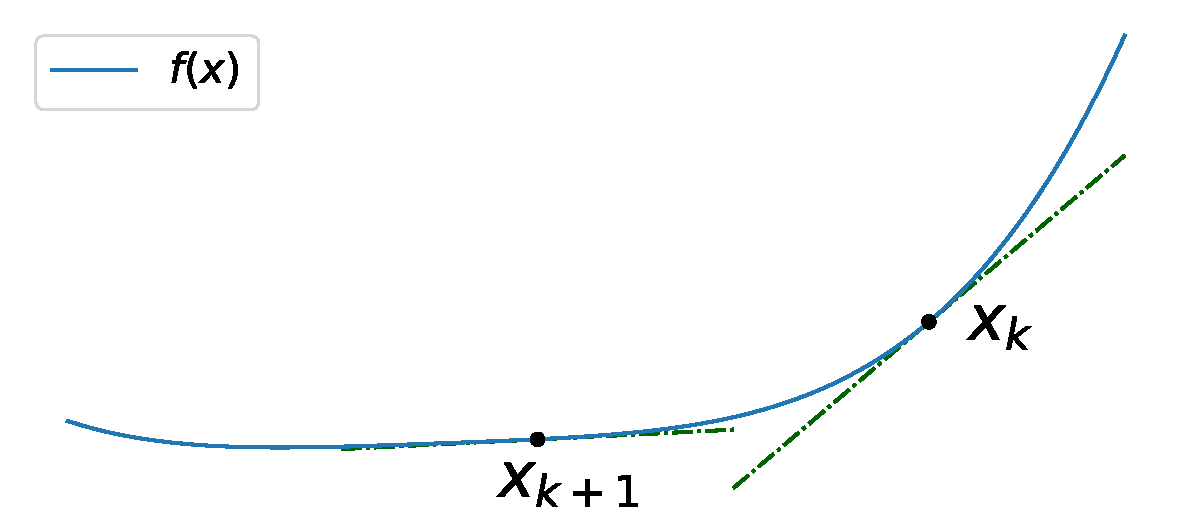
\includegraphics[width=\linewidth]{../imgs/modified_secant/trial_EXPLAIN.pdf}
        \subcaption{Available function and gradient data at $x_k$ and $x_{k+1}$.}
        \label{fig:msec_explain}
    \end{subfigure}%
    \hfill
    \begin{subfigure}[t]{0.33\textwidth}
        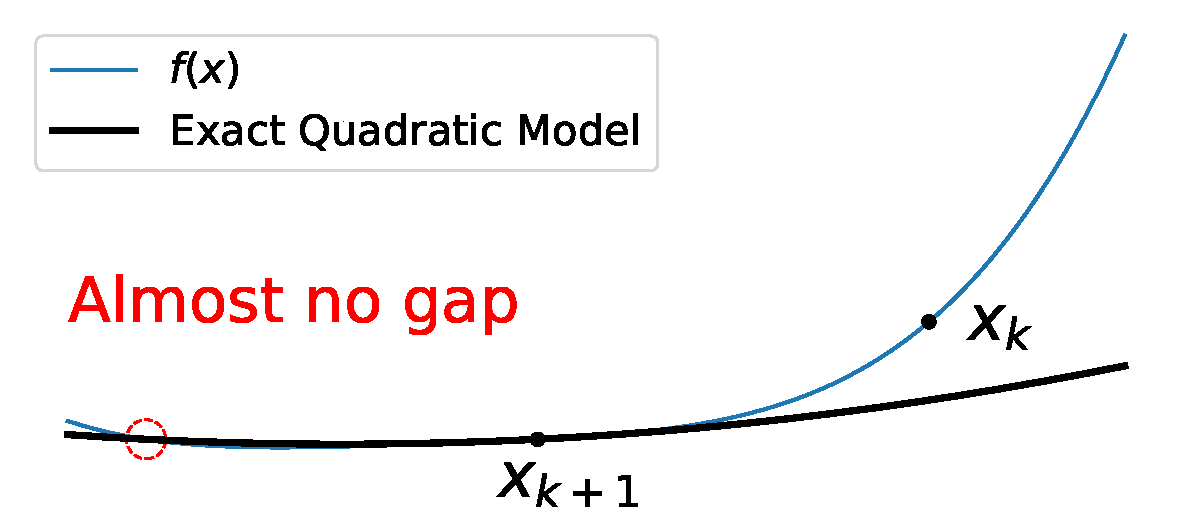
\includegraphics[width=\linewidth]{../imgs/modified_secant/trial_HESS.pdf}
        \subcaption{Ideal quadratic from the exact Hessian.}
        \label{fig:ideal_model}
    \end{subfigure}%
    \hfill
    \begin{subfigure}[t]{0.33\textwidth}
        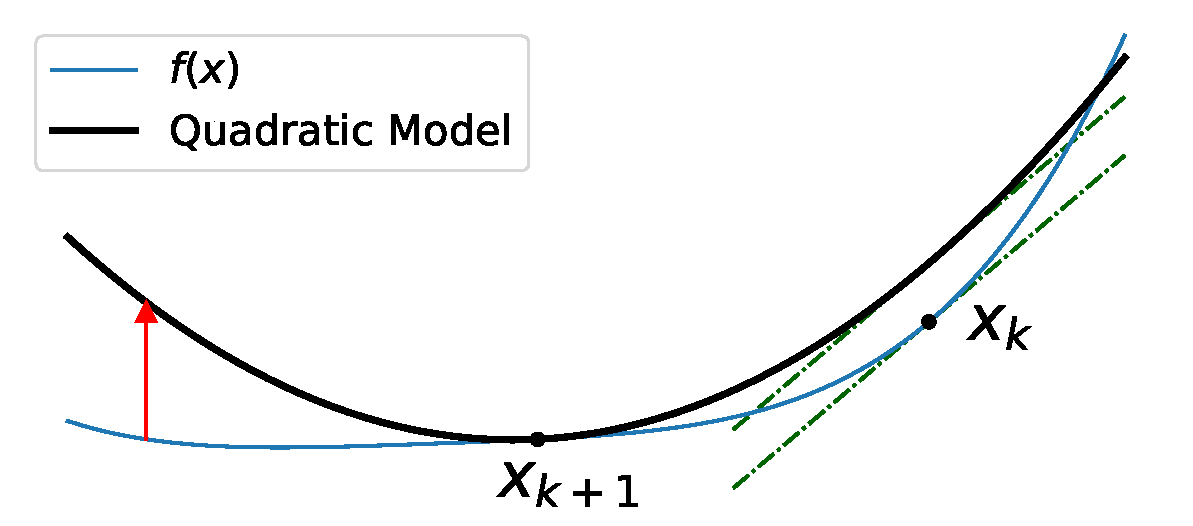
\includegraphics[width=\linewidth]{../imgs/modified_secant/trial_BFGS.pdf}
        \subcaption{Standard secant matches gradient but not $f(x_k)$.}
        \label{fig:standard_secant}
    \end{subfigure}
    \caption{Motivation for modified secant equations. Combining function values with gradients (a) aims to approximate the ideal Newton model (b), while the standard secant update (c) omits $f(x_k)$ and can misestimate curvature.}
    \label{fig:msec_overview}
\end{figure}

We can overcome this limitation by utilizing the function values.
The basic idea is illustrated in \cref{fig:cubic_interpolation}.
Even when the gradients are the same at two points $x_k$ and $x_{k+1}$, natural interpolation of function values differs depending on the function values $f(x_k)$ and $f(x_{k+1})$.
This observation motivates the modified secant condition, which incorporates function value information to improve Hessian approximation.

\begin{figure}[htbp]
    \centering
    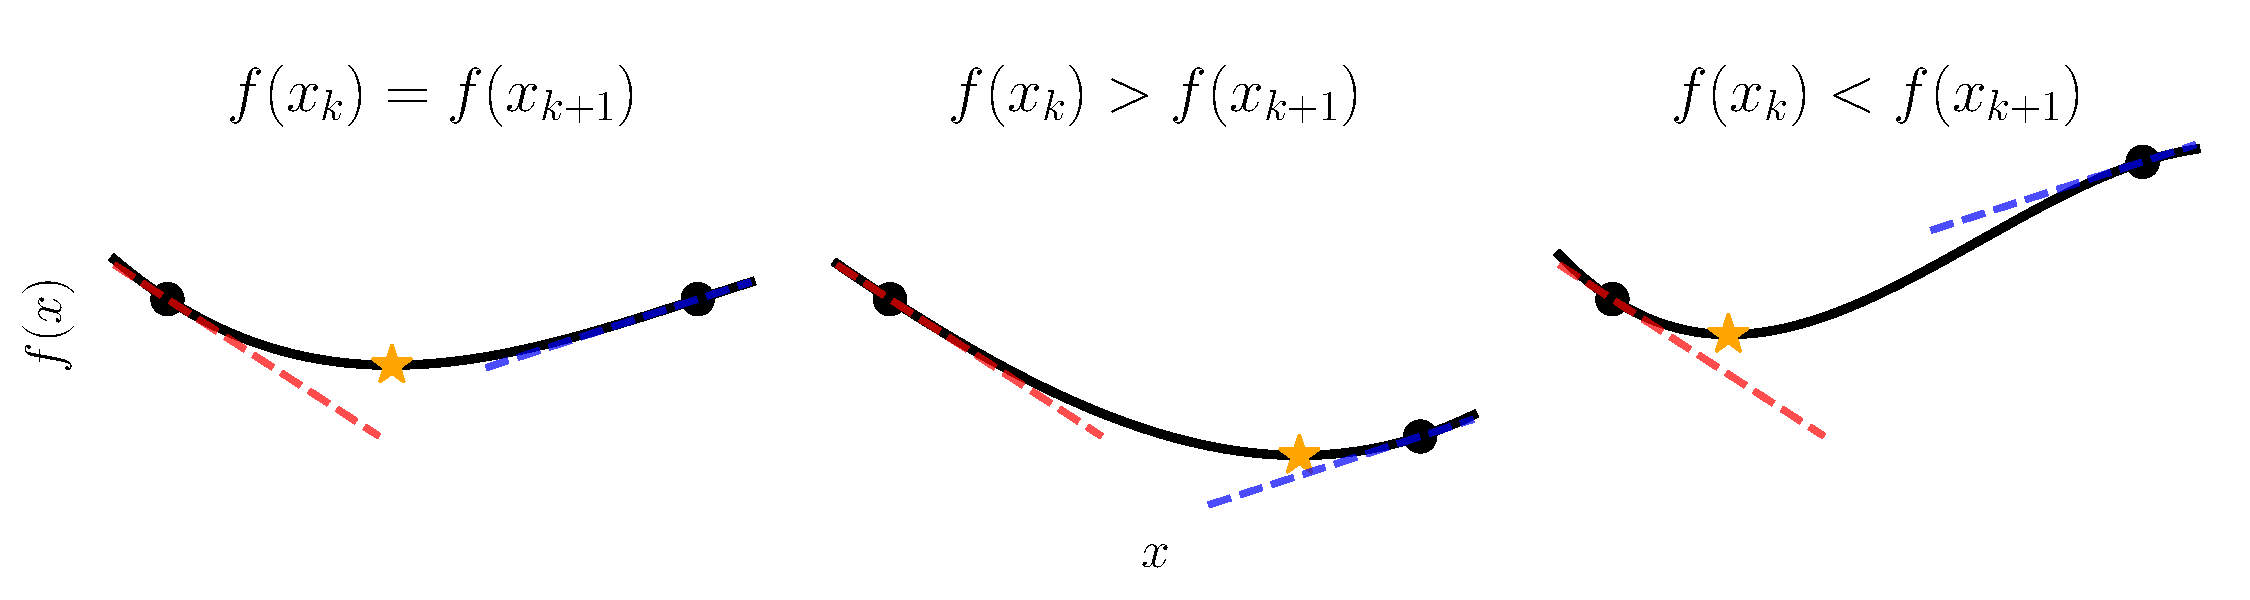
\includegraphics[width=\textwidth]{../imgs/modified_secant/cubic_interpolation.pdf}
    \caption{Interpolation with identical gradients at $x_k$ and $x_{k+1}$ but different function values.
        This leads to distinct interpolants, highlighting the importance of incorporating function value information in Hessian approximation.}
    \label{fig:cubic_interpolation}
\end{figure}

In the following, we present two well-known modified secant conditions.

\subsubsection{Function-Value-Based Modified Secant Condition}
\label{subsubsec:yuan}

The first modification incorporates the function value at the previous point into the quadratic model \citep{yuanModifiedBFGSAlgorithm1991,weiNewQuasiNewtonMethods2006, babaie-kafakiModifiedBFGSAlgorithm2011}.
Let us consider an alternate model with a different approximate Hessian $B^{\mathrm{F}}_{k+1}$:
\begin{equation}
    m_{k+1}^{\mathrm{F}}(x) = f(x_{k+1}) + \nabla f(x_{k+1})^\top (x - x_{k+1}) + \frac{1}{2} (x - x_{k+1})^\top B^{\mathrm{F}}_{k+1} (x - x_{k+1}).
    \label{eq:model_Y}
\end{equation}
In addition to \cref{eq:two_auto_matches}, we require this model to satisfy
\begin{equation}
    m^{\mathrm{F}}_{k+1}(x_k) = f(x_k),
    \label{eq:msecY_fxk}
\end{equation}
which enforces that the function value at the previous point is correctly modeled.
This is the key idea behind function-value-based modified secant conditions.

Let us derive the corresponding modified secant condition for $B^{\mathrm{F}}_{k+1}$.
Substituting the definition of $m^{\mathrm{F}}_{k+1}$ from \cref{eq:model_Y} and using $s_k = x_{k+1} - x_k$ into \cref{eq:msecY_fxk}, the condition becomes
\begin{align}
    f(x_k) & = f(x_{k+1}) + \nabla f(x_{k+1})^\top (x_k - x_{k+1}) + \frac{1}{2} (x_k - x_{k+1})^\top B^{\mathrm{F}}_{k+1} (x_k - x_{k+1}) \notag \\
           & = f(x_{k+1}) - \nabla f(x_{k+1})^\top s_k + \frac{1}{2} s_k^\top B^{\mathrm{F}}_{k+1} s_k. \label{eq:yuan_rearranged}
\end{align}
Now, assume that the updated matrix has the form
\begin{equation}\label{eq:yuan_ansatz}
    B^{\mathrm{F}}_{k+1} s_k = y_k - \sigma^\mathrm{F}_k s_k,
\end{equation}
where $\sigma^\mathrm{F}_k \in \mathbb{R}$ is a scalar to be determined.
Substituting \cref{eq:yuan_ansatz} into \cref{eq:yuan_rearranged} and using $s_k^\top B^{\mathrm{F}}_{k+1} s_k = s_k^\top y_k - \sigma^\mathrm{F}_k \norm{s_k}^2$ gives
\begin{equation}\label{eq:yuan_substituted}
    f(x_k) = f(x_{k+1}) - \nabla f(x_{k+1})^\top s_k + \frac{1}{2} s_k^\top y_k - \frac{\sigma^\mathrm{F}_k}{2} \norm{s_k}^2.
\end{equation}
Solving for $\sigma^\mathrm{F}_k$ and using $y_k = \nabla f(x_{k+1}) - \nabla f(x_k)$, we obtain
\begin{align}
    \sigma^\mathrm{F}_k & = \frac{2(f(x_{k+1}) - f(x_k)) - (2\nabla f(x_{k+1}) - y_k)^\top s_k}{\norm{s_k}^2}           \\
                        & = \frac{2(f(x_{k+1}) - f(x_k)) - (\nabla f(x_{k+1}) + \nabla f(x_k))^\top s_k}{\norm{s_k}^2}.
    \label{eq:C_simplified}
\end{align}
Therefore, the modified secant condition \cref{eq:yuan_ansatz} becomes
\begin{equation}
    B^{\mathrm{F}}_{k+1} s_k = y_k + \frac{2(f(x_k) - f(x_{k+1})) + (\nabla f(x_{k+1}) + \nabla f(x_k))^\top s_k}{\norm{s_k}^2} s_k.
    \label{eq:msecY_raw}
\end{equation}
To preserve the possibility of maintaining positive definiteness under a BFGS-type update when $s_k^\top y_k > 0$, we can modify the formula by taking the maximum with zero in the numerator.
\begin{equation}
    B^{\mathrm{F}'}_{k+1} s_k = y_k + \frac{\max(0, 2(f(x_k) - f(x_{k+1})) + (\nabla f(x_{k+1}) + \nabla f(x_k))^\top s_k)}{\norm{s_k}^2} s_k.
    \label{eq:msecY_final}
\end{equation}

This is the function-value-based modified secant condition.
Unlike the standard secant condition, this formulation ensures that the quadratic model matches not only the function value at the previous point but also the gradients at both points.
Refer to \cref{fig:yuan_msec} for an illustration.

\begin{figure}[t]
    \centering
    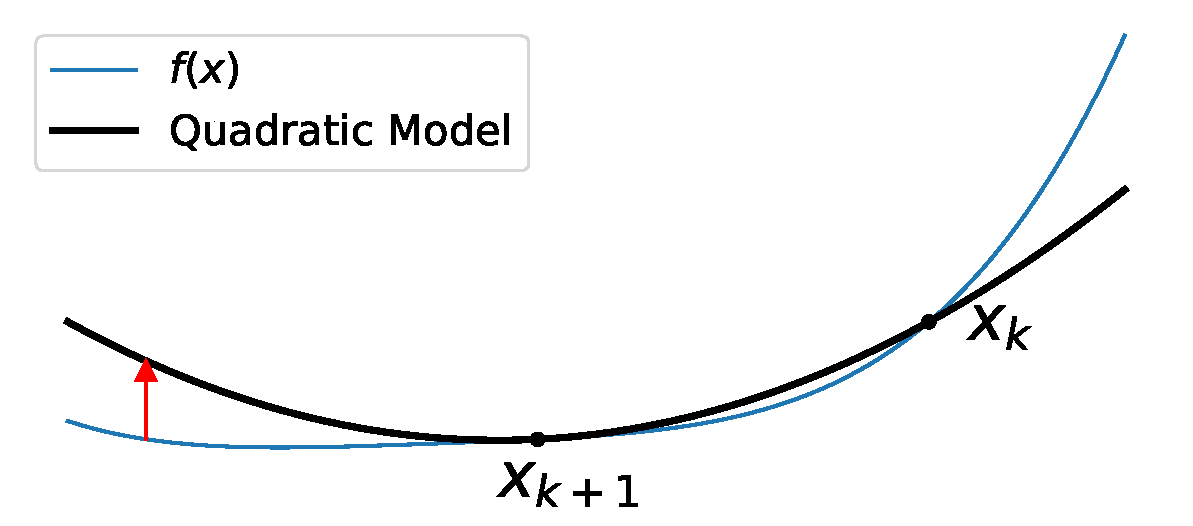
\includegraphics[width=0.7\textwidth]{../imgs/modified_secant/trial_2.pdf}
    \caption{Function-value-based modified secant equation. The modified secant equation $B^\mathrm{F}_k s_k = y_k + \sigma^\mathrm{F}_k s_k$ constructs a quadratic model that satisfies the function value condition $m^{\mathrm{F}}_k(x_{k-1}) = f(x_{k-1})$ at the previous point. This differs from the standard secant equation, which only matches gradients but not function values.}
    \label{fig:yuan_msec}
\end{figure}

\subsubsection{Cubic-Augmented Modified Secant Condition}
\label{subsubsec:zhang}

The second modification introduces a cubic term to the model, allowing simultaneous satisfaction of both function value and gradient matching at the previous point \citep{zhangNewQuasiNewtonEquation1999, zhangPropertiesNumericalPerformance2001,yabeLocalSuperlinearConvergence2007}.
Let $T_{k+1} \in \mathbb{R}^{n \times n \times n}$ be the third-order derivative tensor of $f$ at $x_{k+1}$ such that
\begin{equation}
    s_k^\top (T_{k+1} s_k) s_k = \sum_{i,j,l=1}^n \partial_{x_i x_j x_l} f(x_{k+1}) s_k^{(i)} s_k^{(j)} s_k^{(l)},
\end{equation}
where $\partial_{x_i x_j x_l} f$ denotes the third derivative of $f$ with respect to $x_i$, $x_j$, and $x_l$, and $s_k^{(i)}$ is the $i$-th component of the vector $s_k$.
We introduced this tensor solely for analysis purposes, and it will be eliminated from the final formula.

By incorporating this tensor term, we can define the following cubic-augmented model:
\begin{multline}
    m^\mathrm{C}_{k+1}(x) = f(x_{k+1}) + \nabla f(x_{k+1})^\top (x - x_{k+1}) + \frac{1}{2} (x - x_{k+1})^\top B_{k+1}^{\mathrm{C}} (x - x_{k+1})\\ + \frac{1}{6}(x - x_{k+1})^\top (T_{k+1} (x - x_{k+1})) (x - x_{k+1}).
    \label{eq:model_Z}
\end{multline}
With this model, we can enforce both function value and gradient matching at the previous point $x_k$.
Specifically, we require
\begin{equation}
    \begin{dcases}
        m^\mathrm{C}_{k+1}(x_k) = f(x_k) \\
        \nabla m^\mathrm{C}_{k+1}(x_k) = \nabla f(x_k)
    \end{dcases}
    \label{eq:msecZ_xk}
\end{equation}
By substituting the definition of $m^\mathrm{C}_{k+1}$ from \cref{eq:model_Z} and using $s_k = x_{k+1} - x_k$, we can rewrite these conditions as
\begin{align}
    f(x_k)        & = f(x_{k+1}) - s_k^\top \nabla f(x_{k+1}) + \frac{1}{2} s_k^\top B^\mathrm{C}_{k+1} s_k - \frac{1}{6} s_k^\top (T_{k+1} s_k) s_k,  \label{eq:zhang_func_eq} \\
    \nabla f(x_k) & = \nabla f(x_{k+1}) - B^\mathrm{C}_{k+1} s_k + \frac{1}{2} (T_{k+1} s_k) s_k.
    \label{eq:zhang_grad_eq}
\end{align}
Rearranging \cref{eq:zhang_func_eq} and projecting \cref{eq:zhang_grad_eq} onto $s_k$ gives
\begin{align}
    3(f(x_k) - f(x_{k+1})) +3 s_k^\top \nabla f(x_{k+1}) & = \frac{3}{2} s_k^\top B^{\mathrm{C}}_{k+1} s_k - \frac{1}{2} s_k^\top (T_{k+1} s_k) s_k, \label{eq:zhang_func_rearranged} \\
    -s_k^\top y_k                                        & = -s_k^\top B^{\mathrm{C}}_{k+1} s_k + \frac{1}{2} s_k^\top (T_{k+1} s_k) s_k. \label{eq:zhang_grad_projected}
\end{align}
By summing up \cref{eq:zhang_func_rearranged,eq:zhang_grad_projected} and using $y_k = \nabla f(x_{k+1}) - \nabla f(x_k)$, we eliminate the tensor term and obtain the scalar identity
\begin{equation}
    3(f(x_k) - f(x_{k+1}))
    + \frac{3}{2} s_k^\top (\nabla f(x_{k+1}) + \nabla f(x_k)) + \frac{1}{2} s_k^\top y_k
    = \frac{1}{2} s_k^\top B^{\mathrm{C}}_{k+1} s_k.
    \label{eq:zhang_scalar_identity}
\end{equation}
Assume again that $B^{\mathrm{C}}_{k+1} s_k$ is a linear combination of $y_k$ and $s_k$, i.e., $B^{\mathrm{C}}_{k+1} s_k = y_k + \sigma^\mathrm{C}_k s_k$ for some scalar $\sigma^\mathrm{C}_k$.
Then, \cref{eq:zhang_scalar_identity} yields
\begin{equation}
    \sigma^\mathrm{C}_k = \frac{6(f(x_k) - f(x_{k+1})) + 3 s_k^\top (\nabla f(x_k) + \nabla f(x_{k+1}))}{\norm{s_k}^2}.
    \label{eq:sigma_scalar}
\end{equation}
Plugging \cref{eq:sigma_scalar} back into the ansatz yields the cubic-augmented modified secant condition:
\begin{equation}\label{eq:msecZ_final}
    B^{\mathrm{C}}_{k+1} s_k = y_k + \frac{6(f(x_k) - f(x_{k+1})) + 3 s_k^\top (\nabla f(x_k) + \nabla f(x_{k+1}))}{\norm{s_k}^2} s_k.
\end{equation}

This is a cubic-augmented modified secant condition. Unlike the function-value-based quadratic modification, this formulation allows simultaneous satisfaction of both the function value and gradient conditions at the previous point through the introduction of the tensor term.
Refer to \cref{fig:zhang_models} for an illustration.

\begin{figure}[t]
    \centering
    \begin{subfigure}[t]{0.49\textwidth}
        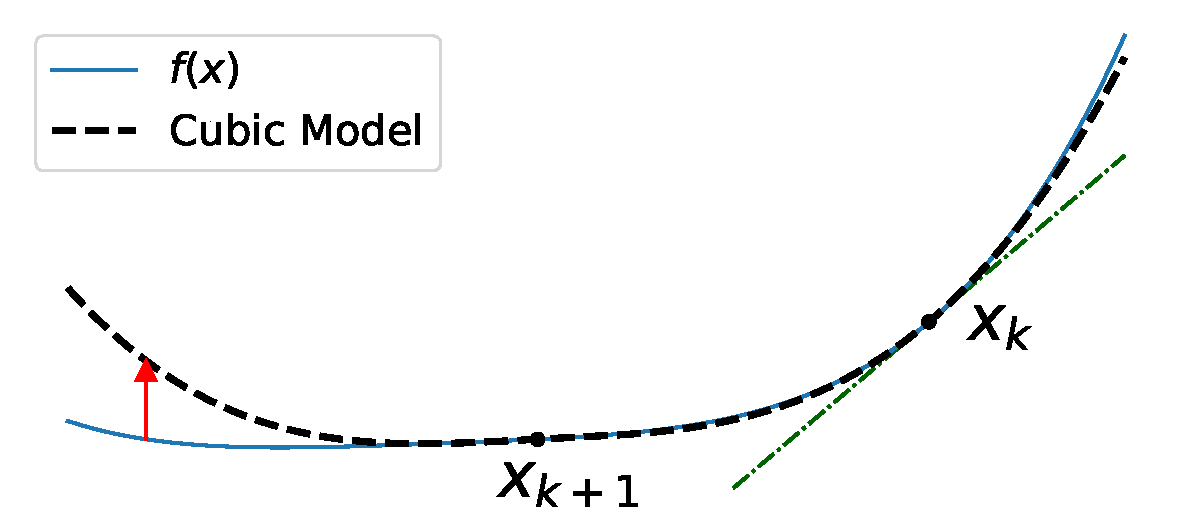
\includegraphics[width=\linewidth]{../imgs/modified_secant/trial_1_cubic.pdf}
        \subcaption{Cubic-augmented modified secant.}
        \label{fig:zhang_cubic}
    \end{subfigure}%
    \hfill
    \begin{subfigure}[t]{0.49\textwidth}
        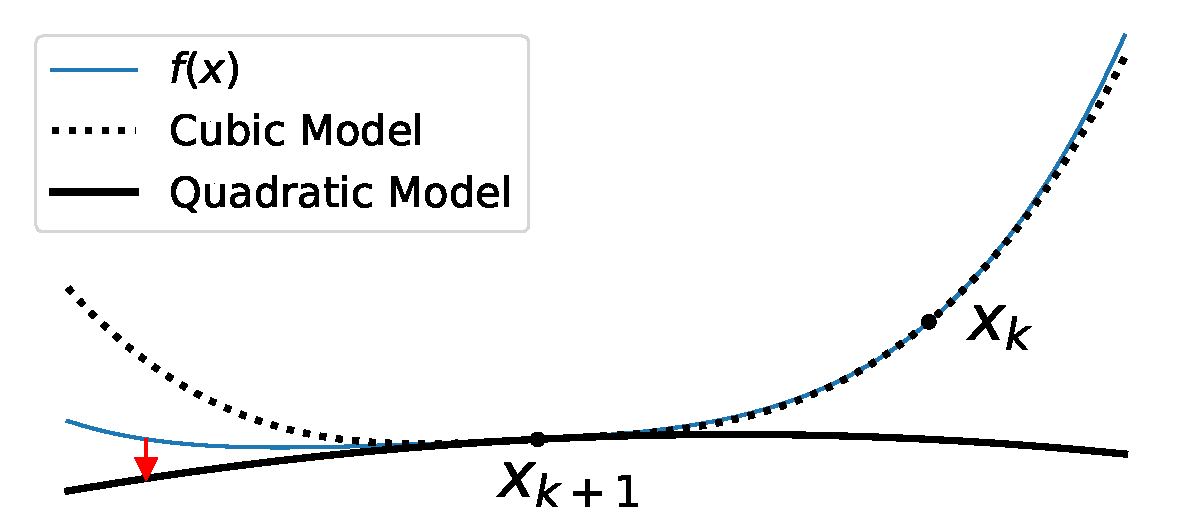
\includegraphics[width=\linewidth]{../imgs/modified_secant/trial_1_quadratic.pdf}
        \subcaption{Quadratic expansion of the cubic-augmented model.}
        \label{fig:zhang_quadratic}
    \end{subfigure}
    \caption{Cubic-augmented modified secant equation.
        In \cref{fig:zhang_cubic}, by incorporating a cubic term $\eta \norm{x - x_k}^3$ in the model, the modified secant equation $B^\mathrm{C}_k s_k = y_k + \sigma^\mathrm{C}_k s_k$ enables simultaneous satisfaction of both conditions at the previous point.
        In \cref{fig:zhang_quadratic}, while the cubic model satisfies both function value and gradient conditions, its underlying quadratic component may be indefinite or negative definite.}
    \label{fig:zhang_models}
\end{figure}

\subsection{Other Curvature Storage Methods}

For storing the curvature information, there are several topics.
Agg-BFGS \citep{berahasLimitedmemoryBFGSDisplacement2022} is an alternative approach to managing curvature information by aggregating data rather than discarding the oldest information and adding the newest.
Multi-Secant \citep{leeAdvancingMultiSecantQuasiNewton2025} extends the secant condition framework by maintaining multiple pairs of step and gradient difference vectors. In the standard formulation, we define
\begin{equation*}
    s_i = x_{i+1} - x_i, \quad y_i = \nabla f(x_{i+1}) - \nabla f(x_i). \quad (i = k-m, \ldots, k)
\end{equation*}
An alternative anchored formulation centers all vectors at the most recent iterate:
\begin{equation*}
    s_i = x_{k+1} - x_i, \quad y_i = \nabla f(x_{k+1}) - \nabla f(x_i). \quad (i = k-m, \ldots, k)
\end{equation*}
This anchored approach provides a different perspective on utilizing historical information for improved Hessian approximation.

\ifSubfilesClassLoaded{
    \bibliographystyle{plainnat}
    \bibliography{../L-BFGS.bib}
}{}

\end{document}
